\section{Project Update}

FANS development is going well despite being slightly behind schedule. The team has a prototype design for a GUI,
multiple diagrams on the systems interactions, and code for some sensory data (temperature). The milestones the team
set are achievable, but we are bound to meet some roadblocks given the amount of work and reports we need to write
outside of developing the system. Time management will be an asset in this project.

Each team member's assigned workload is manageable, and development will pick up once we have access to components
needed for FANS. The only changes to the initial plan will be further extending the time needed to reach each of our
objectives (the objectives themselves are still achievable).

\subsection{Project Milestones}

FANS will continue to be built gradually over the course of the semester, adding new components and interactivity over
time. To better match the team’s workflow and pace, we decided to extend the deadlines for our milestones. By moving
each date up by 1 week, we give ourselves more time to complete the system while staying on schedule.

\begin{table}[H]
    \begin{tabular}{| p{3cm} | c | c | p{7cm} |}
        \hline
        \textbf{Milestone}                           & \textbf{Status} & \textbf{Date}  & \textbf{Description}                                                                                                         \\
        \hline
        Create user-friendly web interface                & In Progress     & Wed March 13th & Develop a user-friendly web interface for monitoring system status, configuring thresholds, and interacting with the system. \\
        \hline
        Establish database for storing system data        & In Progress     & Fri March 16th & Set up a database to store employee
        contact information and system data, ensuring efficient management and retrieval.                                                                                                                                   \\
        \hline
        Develop and test smoke detection algorithm        & Pending Action  & Tue March 19th & Develop and test the smoke
        detection algorithm on the Raspberry Pi to ensure accurate detection of fire and smoke.                                                                                                                             \\
        \hline
        Integrate sensors with Raspberry Pi               & In Progress     & Tue March 26th & Integrate sensors with the Raspberry Pi for
        real-time data collection, enabling the system to monitor environmental conditions.                                                                                                                                 \\
        \hline
        Implement notification system                     & Pending Action  & Sat March 30th & Implement a notification system to trigger
        alarms and alert users via SMS and email in case of fire emergencies.                                                                                                                                               \\
        \hline
        Test functionality of hardware and software       & Pending Action  & Wed April 3rd  & Conduct comprehensive testing to
        ensure the functionality and integration of both hardware and software components.                                                                                                                                  \\
        \hline
        Finalize system configuration and conduct testing & Pending Action  & Fri April 5th  & Finalize system
        configuration, including thresholds and notification settings, and conduct comprehensive testing.                                                                                                                   \\
        \hline
    \end{tabular}
    \caption{Project milestones for the development of FANS.}
\end{table}

\subsection{Schedule of Activities}

Figure \ref{fig:timeline} below is an updated Gantt chart showing the new deadlines for our various milestones. The
status of "In Progress" and "Completed" activities are shown in the diagram using icons.

\begin{figure}[H]
    \centering
    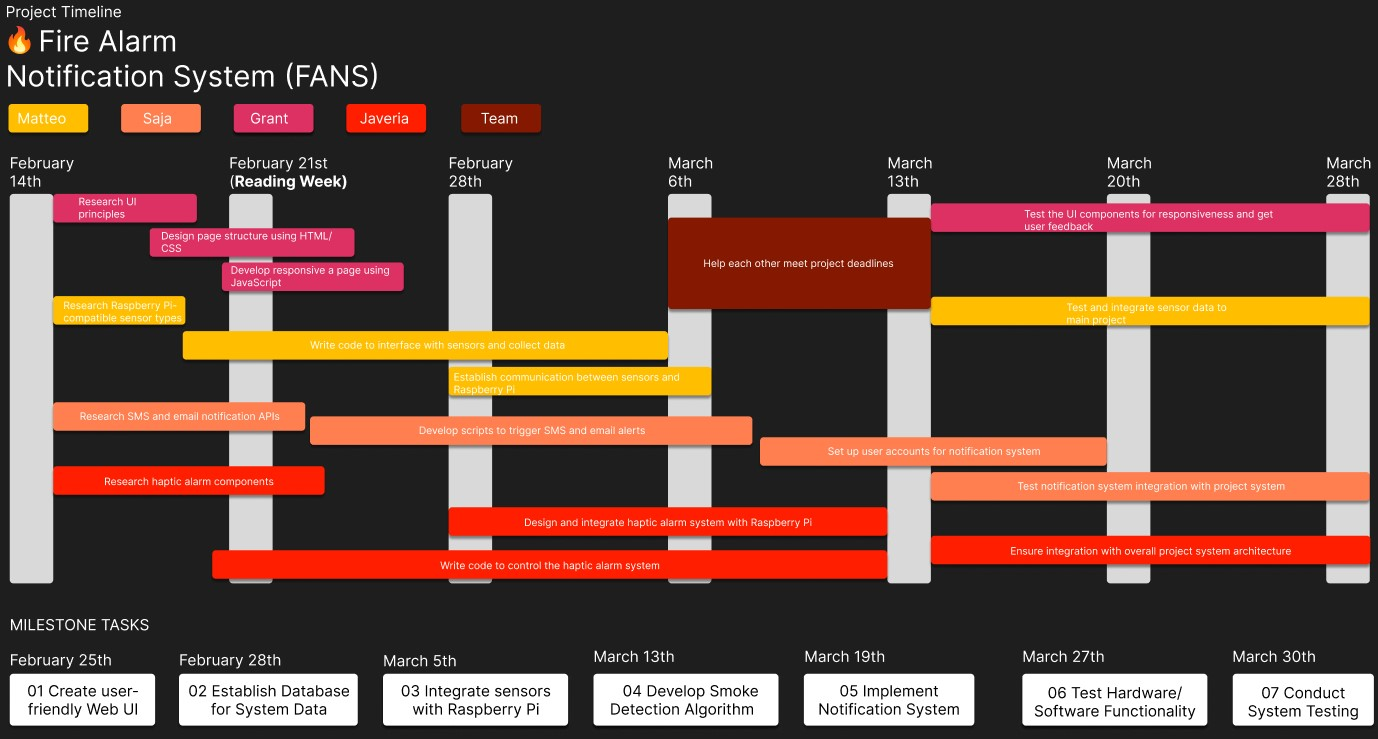
\includegraphics[width=\linewidth]{../assets/SYSC3010_ProjectTimeline.jpg}
    \caption{Timeline for FANS development.}
    \label{fig:timeline}
\end{figure}
